\documentclass[11pt,leqno,oneside]{amsart}
%\usepackage[margin=1in]{geometry}

\usepackage{../notes}
\usepackage{xfrac}
\usepackage{enumitem}
\usepackage{tikz-cd}
\usetikzlibrary{cd}
\usepackage{hyperref}
\usepackage{amsrefs} % AMS references % must be loaded AFTER hyperref if you use that
\usepackage{mathtools}
\mathtoolsset{showonlyrefs}

\usepackage{datetime}
% an environment specifically for my dates, although it doesn't actually depend on datetime:
\newenvironment{dateenv}{
  \vspace{1em}
}{
  \vspace{1em}
}
% my date command, for convenient date adding
\newcommand{\mydate}[4]{
  \newdate{#1}{#2}{#3}{#4}
  % #1 is a unique string, #2 is day, #3 month, #4 year
  \begin{dateenv}
    \hfill\displaydate{#1}
  \end{dateenv}
}

\numberwithin{thm}{section}
\setlength\parindent{0pt}

\everymath{\displaystyle}

\newcommand{\minus}{\smallsetminus}
\renewcommand{\setminus}{\smallsetminus}
\renewcommand{\amalg}{\sqcup}
\newcommand{\homotopic}{\simeq}
\renewcommand{\epsilon}{\varepsilon}
\renewcommand{\d}{\partial}
\newcommand{\fund}{\pi_1}
\newcommand{\transverse}{\pitchfork}
\newcommand{\x}{\times}
\newcommand{\Map}{\text{Map}}
\newcommand{\id}{\text{id}}
\renewcommand{\bar}{\widebar}

%%%%%%%%%%%%%% BEGIN CONTENT: %%%%%%%%%%%%%%

\title[Algebraic Topology]{Algebraic Topology MATH 7800}
\author{Chris Lloyd, Matthew Lancellotti}
\date{}
\begin{document}
\maketitle \newpage

\mydate{d1}{18}{1}{2017}

\section{Introduction}

Topology is floppy. Given just a topological space one has an infinite
degree of freedom. This makes even simple questions hard to answer, in
particular given manifolds \(M\) and \(N\) with different dimensions
\(m\) and \(n\) respectively, one may ask if they are
homeomorphic. Intuitively one would think that should not be
possible. However there do exist space filling curves, i.e,
\[I \twoheadrightarrow I \times I\]
where as always \(I=[0,1]\).

We will develop the tools to prove manifolds of different dimensions can
certainly never be homeomorphic. Another surface result assures there exists no continuous
retraction \(D^2 \to \d D^2\), which then immediately yields the
Brouwer Fixed Pointed Theorem (every map \(D^2 \to D^2\) admits a
fixed point).

In this course there will be two basic branches under consideration:
homotopy theory and homology. Basically, homotopy concerns itself with
continuous deformations between maps. While homology studies subspaces
(known as ``cycles'') and gap filling.

\section{Reference}
%
\begin{defn}
  $D^n$ denotes the $n$-dimensional closed unit disk.
\end{defn}

\section{Homotopy}

We now define homotopies in the space of maps between manifolds \(M\)
and \(N\) denoted
\[\Map(M,N)=\{f \from M \to N \mid \text{$f$ is continuous}\}.\]

In this course, we follow the convention that maps are continuous
functions unless otherwise stated!

\begin{defn}
  A \emph{homotopy} from \(f \in \Map(M, N)\) to \(g \in \Map(M, N)\) is a path in $\Map(M, N)$ that starts at $f$ and ends at $g$.  Therefore, $h_0 = f$ and $h_1 = g$.

  Equivalently, a \emph{homotopy} from \(f \from M \to N\) to \(g \from M \to N\)
  is a map \(h\from M \x I \to N\) such that \(h_0=f\) and \(h_1=g\). We say \(f\) and
  \(g\) are \emph{homotopic} if a homotopy between them exists.

  Often we write \(h_t(m)\) for \(h(m,t)\).
\end{defn}

When working with homotopies one often thinks of having the start and
end map already fixed. For maps to be homotopic they must be in the
same path component.

\begin{prop}
  Homotopy is an equivalence relation.
\end{prop}

We denote the homotopy equivalence class of \(f\) by \([f]\).

\begin{defn}
  A homotopy $h\from I \x X \to Y$ is called \de{relative} to a subset $A$ of $X$ if for all $a \in A$ and all $t \in I$, $h(a, t) = f(a) = g(a)$.

  We also say that ``$f$ and $g$ are homotopic relative to $A$''.
\end{defn}

When there are no restrictions placed on a homotopy, it is sometimes called a \emph{free} homotopy.

\begin{defn}
  A \emph{path} in a topological space $X$ is a map
  \[f \from I \to X.\]
\end{defn}

By convention in this course, we always consider paths up to homotopy relative to $\{0, 1\}$.  That means that our homotopies fix the end points.  If they didn't, every path would collapse to a point up to homotopy!

Imagine two paths in \(\R^2 \setminus (0,0)\) which agree on end points,
however each path is on opposite sides of the origin. It is clear that
there exists no end point fixing homotopy between the two paths.

\begin{defn}
  If one has two paths \(f,g\) with \(f(1)=g(0)\) we may define a new
  path
  \[f * g :=
    \begin{cases}
      f(2t), & t \in [0,\frac{1}{2})\\
      g(2t - 1), & t \in [\frac{1}{2},1].
    \end{cases}
  \]

  This is called the \emph{concatenation} or \emph{path composition}
  of $f$ and $g$.

  This operation is well defined on homotopy classes, that is if
  \([f]=[f']\) and \([g]=[g']\) then \([f * g] = [f' * g']\). This
  operation may be generalized to \(*_{k}\) where \(k \in (0,1)\),
  simply replace \(\frac{1}{2}\) with \(k\). In this notation
  \(f * g = f *_{\frac{1}{2}} g\). Concatenation is associative.
\end{defn}

Given a topological space \(X\) with points \(P\), for any two points
\(x,y \in P\) we have a set of homotopy classes with end points \(x\)
and \(y\). These may be thought of as morphisms and the points as
objects in a category. We call this category the Fundamental Groupoid.

\mydate{d2}{20}{1}{2017}

\begin{defn}[\cite{ncatlab}]
  A \de{category} $\mathcal{C}$ consists of
  \begin{itemize}
    \item A class of objects $\Ob(\mathcal{C})$
    \item For every pair of objects $A, B \in \Ob(\mathcal{C})$, a set $\Hom(A, B)$ of \de{morhpisms}
    \item A composition operation.  That is, if $f \in \Hom(A,B)$ and $g \in \Hom(B,C)$, then there exists a morphism $h \in \Hom(A,C)$ s.t. $h = f.g$, where ``.'' denotes the composition operation.  The composition operation must be associative.
    \item For every object $A \in \Ob(\mathcal{C})$, an \de{identity morphism} $\id_A\from A \to A$ s.t. for all $f\from A \to B$ we have $\id_A.f = f$ and for all $g\from B \to A$ we have $g.\id_A = g$, for all $B$.
  \end{itemize}
\end{defn}

\begin{defn}
  In the category of \de{finite sets}, denoted $\text{FSet}$, the
  objects are the finite sets, each morphism from $A$ to $B$ is a
  function from $A$ to $B$.
\end{defn}
\begin{defn}
  For any field $K$, the category of \de{$K$-vector spaces} (vector spaces over $K$), denoted
  $\text{Vect}_K$, has objects that are $K$-vector spaces and
  morphisms that are $K$-linear maps.
\end{defn}
\begin{defn}
  A \de{groupoid} is a category where every morphism has an inverse.

  That is, for any objects $x$ and $x'$ and any morphism $a \from x \to x'$ between them, there exists $a^{-1} \from x' \to x$
  s.t. $aa^{-1} = \id_{x'}$ and $a^{-1}a = \id_{x}$.
\end{defn}
\begin{rmk}
  A groupoid can be viewed as a more general notion than a group!

  The elements of the groupoid are the morphisms.  The operation is composition.  Not every pair of morphisms can necessarily be composed!

  So a groupoid is just like a group, but not every pair of elements can be multiplied!  Also, there is not a \textbf{single} identity, but rather, there could be many left and right identities.  That is, each object has a little loop.
\end{rmk}
\begin{prop}
  Every morphism in a groupoid is an isomorphism (by definition).
\end{prop}
\begin{defn}
  A \de{group} is a groupoid with one object.
\end{defn}
\begin{prop}
  If $A$ is an object in a groupoid, then $\Hom(A, A)$ is a group.
\end{prop}

Note, we see that a groupoid is the same definition of a group, but we
use a *partial* binary operation instead of a binary operation.

\begin{defn}
  The \de{fundamental groupoid} of $X$, denoted $\Pi_1 X$, is the
  category where the objects are the points in $X$ and the morphisms
  are the paths (up to endpoint fixing homotopy) between those points.
\end{defn}
\begin{defn}
  The \de{fundamental group of $X$ at the basepoint $x_0$}, denoted
  $\pi_1(X, x_0)$, is the subgroupoid of the fundamental groupoid
  where there is exactly one object, $x_0$, and the morphisms are the
  morphisms of the fundamental groupoid that have source and target
  $x_0$.  Another wording is to say that $\pi_1(X, x_0)$ is the full
  subcategory of $\Pi_1 X$ spanned by $x_0$.

  The elements of the group are the morphisms.  The operation is
  composition.
\end{defn}
\begin{defn}
  The \de{inverse path} of a path $p$ is $p^{-1}(s) := p(1-s)$.  In Hatcher, this is denoted $\bar{p}$.
  (Note: This is *not* the same as the function inverse of $p$)
\end{defn}
\begin{prop}
  If $p$ is a path, then
  $[p^{-1}*p] = [id_{x}]$, which is the equivalence class of the
  function where $s \mapsto x$ for
  all $s \in [0,1]$.
\end{prop}

\begin{thm}[Hatcher 1.5]
  Let $X$ be a metric space and $x,x' \in X$.  If there exists
  $p\from x \to x'$ and $[q] \in \pi_1(X,x')$, then
  $p^{-1}qp \in \pi_1(X,x)$.  The ``conjugacy'' map that sends each $[q]$ to $[p^{-1}qp]$ is an isomorphism of fundamental groups.
\end{thm}
\begin{thm}
  If $X$ is path connected, then for any $x_a, x_b \in X$,
  $$\pi_1(X, x_a) \isom \pi_1(X, x_b).$$
\end{thm}
In the above situation, we can denote the fundamental
group with $\pi_1(X)$ or $\pi_1 X$.
\begin{example}
  pretty picture %

  This isomorphism is not canonical


  Note that $\pi_1 X$ is only well defined up to inner automorphism.
\end{example}
\begin{defn}
  Given spaces $X, Y$ and a map $f\from X \to Y$, then the
  \de{fundamental functor} induced by $f$,
  $$f_* = \Pi_1 f \from \Pi_1 X \to \Pi_1 Y$$ maps each object $x \in X$
  to $f(x) \in Y$ and each path $[p] \in \Pi_1 X$ to
  $f([p]) = [f(p)] \in \Pi_1 Y$.
\end{defn}
\begin{prop}
  The above is well defined because
  \begin{itemize}
  \item If $[p]=[q]$, then $[f(p)] = [f(q)]$.  Proof:  Consider the homotopy $h$ s.t. $h_0 = p$ and $h_1 = q$.  $f$ is continuous, so $h.f$ is a homotopy, and $(h.f)_0 = f(p)$ and $(h.f)_1 = f(q)$.
  \item If $p$ and $q$ represent equivalence classes, and if they can be concatenated, then $(f_*p)*(f_*q) = f_*(p*q)$.
  \end{itemize}
\end{prop}

\begin{prop}
  Given a fundamental group $\fund(X, x)$, then we can restrict $f_*$
  to the functor $$f_* \from \fund(X, x) \to \fund(Y, f(x)).$$ which is a group homomorphism.

  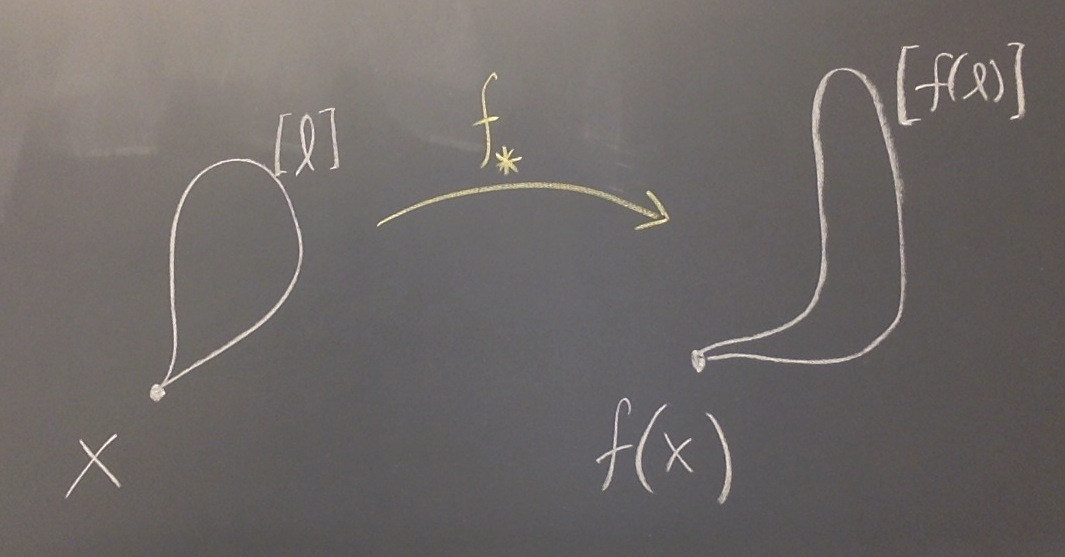
\includegraphics[scale=0.17]{images/fundamental-functor}
\end{prop}
\begin{prop}
  If $X,Y,Z$ are metric spaces and $f \from X \to Y$, $g \from Y \to Z$ are
  maps, then ${(f.g)}_* = f_*.g_*$.
\end{prop}

\begin{example}
  $\fund(\R^n, x) = \{[*]\} = \{e\}$

  In $\Pi_1 \R^n$, there exists a unique path between any two points,
  up to homotopy.

  Note that $\fund(B_n) = \{e\}$ and $\fund(I_n) = \{e\}$ too!
\end{example}
\begin{proof}
  Let $p,q \from I \to \R^n$ be any two paths that satisfy $p(0) = q(0)$ and $p(1) = q(1)$.

  Define $h$ by $h_t = tp + (1-t)q$.  It follows that, $h_0 = q$, $h_1 = p$, and $h$ is a homotopy.
\end{proof}

\begin{defn} % I'm pretty sure this is the DEFINITION of simply connected.  We're just saying "the fundamental group is trivial" instead of saying "every loop can be shrunk continuously to a point".  I suppose we could create a separate definition if you wish.  Also, Hatcher 1.6 doesn't exist.
  A space $X$ is \de{simply connected} or \de{1-connected} iff it is path connected and its
  fundamental group is trivial.
\end{defn}
\begin{example}
  $\R^2 \minus (0,0) \isom \C \minus \{0\}$ is NOT simply connected.
  $\fund(\C \minus \{0\}) = \Z$
\end{example}
\begin{example}
  pretty picture with yellow and blue dots %

  $A$ and $B$ can't be homotopic because $\log(A)$ and $\log(B)$ have
  different end points.
\end{example}

\begin{defn}
  A \emph{covering space} \((\tilde{X},p)\) of a space \(X\) is a space \(\tilde{X}\)
  and map \(p \from \tilde{X} \to X\) where there exists an open cover
  \(\{U_\alpha\}\) of \(X\) and for each $\alpha$, \(p^{-1}(U_\alpha)\) is a
  disjoint union $\dunion V_j$ of open sets in \(\tilde{X}\) such that for all $j$, $p|_{V_j} \from V_j \to U_\alpha$ is a homeomorphism.
\end{defn}

Think of the stack of records theorem from Guillemin and Pollack. See
page 59 in Hatcher for the covering space of two loops as discussed in
class. We now discuss homotopy lifting.

\begin{prop}
  Given a covering space \((\tilde{X},p)\) of \(X\) and a homotopy
  \(h_t \from Y \to X\), and some map
  \(\tilde{f}_0 \from Y \to \tilde{X}\), then there exists a unique
  homotopy \(f_t \from Y \to X\) that lifts \(f_0\), that is
  \begin{center}
    \begin{tikzcd}
      & & \tilde{X}\\
      Y \times \{0\} \arrow[r,hook] \arrow[rru,"\tilde{f}_0", bend
      left]& Y \times I \arrow[r,"f_t",swap] \arrow[ru,dashed,"\tilde{f}_t"]& X \arrow[u,"p"]
    \end{tikzcd}
  \end{center}
\end{prop}

\mydate{d4}{30}{1}{2017}

\section{Functoriality of the fundamental group}

Let $X$, $Y$ be spaces and $f,f' \from X \to Y$ be maps.

We wish to prove (i think) that $f_* \of g_* = (f \of g)_*$.

Let $h\from X \x I \to Y$ be a homotopy from $f$ to $f'$.  In the easy version, we fix a basepoint $x \in X$ and require that $h_t(x)$ is constant. ``based map'' (there exists a category of based spaces, i.e., top w/ fixed point)

$f_* = f'_*$ since $(f \of p) \homotopic (f' \of p)$ via $(h \of p)$.


\begin{thm}
  $$\begin{tikzcd}
    &\fund(X,x) \arrow[r, "f_*"] \arrow[rd, "f'_*"] &\fund(Y,f(x)) \arrow[d, "f_*'(p) = h_t(x) * f_*(p) * h_t(x)^{-1}"] \\
    & &\fund(Y, f'(x))
  \end{tikzcd}$$
  commutes.
\end{thm}
\begin{proof}
  ((chris why wont it let me put pairs in this tikzcd diagram below?))
  $$\begin{tikzcd}
    % &I \x I \arrow[r, "(p,\id)"] &X \x I \arrow[r, "h"] &Y
    &I \x I \arrow[r, ""] &X \x I \arrow[r, "h"] &Y
  \end{tikzcd}$$

  the rectangle is simply connected
  RECTANGLE:
  LEFT
  $f \of p$
  RIGHT
  $f' \of p$
  UP
  $h_t(x)$
  DOWN
  $h_t(x)$

  If $A$ and $B$ are categories and $F,G\from A \to B$ are functors an \underline{isomorphism} of functors.

  For all $a \in \Ob(A)$, $Z(a)\from F(a) \to G(a)$ such that for all $g \from a \to a'$,

  $$\begin{tikzcd}
    &F(a) \arrow[r, "Z(a)"] \arrow[d, "F(g)"] & G(a) \arrow[d, "G(g)"] \\
    &F(a') \arrow[r, "Z(a')"]                  & G(a')
  \end{tikzcd}$$

  ((commutes?))

  Note: if $B$ is a groupoid, any natural transformation is an isomorphism.
\end{proof}

\begin{thm}
  Restatement of above thm

  Given
  $$\begin{tikzcd}
    &X \arrow[r, bend left, "f"] \arrow[r, bend right, "f'"'] &Y
  \end{tikzcd}$$

  where $f \homotopic f'$ via $h$, then

  $$\begin{tikzcd}
    &\Pi(X) \arrow[r, bend left, "f_*"] \arrow[r, bend right, "f_*'"'] &\Pi(Y)
  \end{tikzcd}$$

  and $f_* \isom f_*'$ via the transformation defined by: for all $x \in X$, $h_t(x)\from f(x) \to f'(x)$.
\end{thm}
\begin{defn}
  Given spaces $X$ and $Y$, we call the map $f\from X \to Y$ a \de{homotopy equivalence} if there exists $g\from Y \to X$ s.t. $[f.g] = [\id_X]$ and $[g.f] = [\id_Y]$.
\end{defn}
\begin{rmk}
  Note that $f$ is not a homotopy.  The point is that $f.g$ is homotopic to $\id_X$, and the other way around too.
\end{rmk}
\begin{rmk}
  If $A \into X$ and $A \into Y$, and $f$ as above is a homotopy equivalence relative to $A$ s.t. maps $f,g$ are homotopies must be identity on $A$, then $A = [*]$.

  picture
  sphere torus
  sphere torus

  If $f,g$ are homotopy inverse

  $$\begin{tikzcd}
    &\fund(X,x) \arrow[r, "f", "\isom"'] \arrow[rr, bend right, "\isom", "f.g"'] &\fund(Y, f(x)) \arrow[r, "g", "\isom"'] &\fund(X, g(f(x))
  \end{tikzcd}$$
\end{rmk}
\begin{defn}[retraction, retract, weak deformation retract, strong deformation retract]
  ((these definitions from wolfram mathworld, and they make perfect sense to me))

  For any subspace $A$ of $X$, a \de{retraction} is a map $f\from X \to A$ s.t. for all $a \in A$, $f(a) = a$.

  $A$ is a \de{retract} (of $X$).

  If additionally there exists a homotopy $F\from X \x I \to X$ s.t. $F_0 = \id_X$ and $F_1 = f$, then $A$ is a \de{weak deformation retract}.

  If additionally we have that for all $t \in I$ and all $a \in A$, $F_t(a) = a$, then $A$ is a \de{strong deformation retract}.
\end{defn}
\begin{defn}
  A \de{weak deformation retract} is when you have a homotopy $f\from A \into X$ and a homotopy inverse $g$ s.t. $[g \of f] = [id_A]$ and $[f \of g] = [id_X]$. ((Webster's def))
\end{defn}
\begin{defn}
  A \de{strong deformation retract} is a weak deformation retract where the homotopy inverse is relative to $A$ and $g \of f = \id_A$. ((Webster's def)) ((umm, what does he mean by "relative"?))
\end{defn}
In this class, we follow the convention that \de{deformation retract} refers to strong deformation retract!
\begin{rmk}
  More generally, $g$ is a retraction of $A$ if $g \of f$ = $id_A$. ((Webster's def))
\end{rmk}
\begin{example}
  $S^1 \into \C\minus\{0\}$ is a d.r. where the homotopy is given by $h_w(x) = \frac{x}{|x|^w}$ where $w \in [0,1]$  and $g(x) = \frac{x}{|x|}$.

  ((i infer)) This allows us to conclude that $\fund(\C\minus\{0\}) \isom \fund(S^1)$.
\end{example}
\begin{thm}
  Every map $f\from D^2 \to D^2$ has a fixed point.
\end{thm}



\begin{proof}
  Draw a circle and the points $x$ and $f(x)$.  Draw a ray from $f(x)$ through $x$ that ends at the boundary.  Consider a function $r$ that sends each $x$ to the endpoint of the ray.  This $r$ turns out to be a retraction.  This is our $g\from D^2 \to S^1$.  This is a deformation retract, so by our previous theorem, $\fund(D^2) \isom \fund(S^1)$.  A contradiction.
\end{proof}







\begin{bibdiv}
\begin{biblist}
% THIS SHOULD BE MOVED TO A SEPARATE FILE IF IT GETS TOO CUMBERSOME
% see http://ctan.math.utah.edu/ctan/tex-archive/macros/latex/contrib/amsrefs/amsrdoc.pdf
  \bib{ncatlab}{webpage}{
    title={Joyal's CatLab},
    url={https://ncatlab.org/joyalscatlab/published/Categories},
    accessdate={2017-02-06},
    date={2010-05-30},
  }
\end{biblist}
\end{bibdiv}


\end{document}

%%% Local Variables:
%%% mode: latex
%%% TeX-master: "algebraic-topology.tex"
%%% End:
